\subsection{Physique (coefficient 1)}

\subsubsection{Déroulement de l'épreuve}

L’épreuve de physique est moins guidée que celle de biologie, le professeur te laisse quelques minutes pour réfléchir de ton côté sur un sujet plus ou moins ouvert (en général il y a une à quelques questions pour guider la réflexion), puis tu passes au tableau et commences la résolution. Mais la majeure partie de l’épreuve est surtout une discussion avec l’examinateur qui te pose des questions pour t'orienter à partir du moment où tu bloques.\\

La petite particularité de cette épreuve est que l’examinateur (notre année en tout cas) ne respecte pas tellement les 30 minutes théoriques que dure l’épreuve, ce qui entraîne beaucoup de retard pour les candidats suivants.\\

Théoriquement, le programme comprend l’enseignement de spécialité de terminale en physique-chimie, mais nous te conseillons de maîtriser aussi les notions de première année de médecine et quelques notions de prépa PCSI, le programme de médecine étant différent selon les facultés. Voici une liste des quelques domaines clés à maîtriser qui retombent souvent aux oraux :

\begin{itemize}
\item Optique ondulatoire et optique géométrique de lycée et de PASS, à compléter avec des exercices de prépa
\item Mécanique du point (bilans de forces, travail, vitesse, accélération, $2^e$ loi de Newton...) : programme de lycée et de PASS complété avec des exercices de première année de BCPST ou PCSI (en particulier la résolution des équations différentielles)
\item Mécanique des fluides (principe fondamental de l’hydrostatique, loi des gaz parfaits, loi de Poiseuille, effet Venturi, lois de Hooke et de Laplace, transport membranaire et équilibre de Starling, poussée d’Archimède)
\item Frottements
\item Mécanique des ondes : ondes électromagnétiques et mécaniques, ondes sonores, effet Doppler
\end{itemize}

Il est aussi important de maîtriser les différents outils mathématiques de résolution de problèmes physiques : trigonométrie, géométrie euclidienne de lycée, résolution d’équations différentielles, dérivation...\\

Nous te conseillons aussi de bien t'entraîner sur des exercices de khôlles de prépa puisque l’oral est vraiment du même format. Si tu arrives à te trouver un examinateur qui te fasse passer un oral blanc avec un tableau (un ami en prépa par exemple) c’est l’idéal, puisque tu n’as normalement pas du tout l’habitude de ce format d’épreuve et devoir dérouler son raisonnement sur un tableau pour la première fois le jour J peut parfois être déroutant.

\subsubsection{Témoignages}

\lettrine{{\color{violet} \oldpilcrowfive}}{}
Premier oral de la série. Malgré des horaires assez honnêtes, j'ai encore l'impression de ne pas être totalement sorti de mon lit. Après 5 cafés et 3 passages d'eau glacée sur la tête, je transpire toujours autant mais ne sais toujours pas comment je m'appelle. L'examinateur, très sympa et probablement aussi réveillé que moi m'appelle et il faut y aller : \\

\textbf{Modélisation et analyse d'une pseudo-molécule/noyau et ses électrons}. On étudie 3 masses $m_1, m_2, m_3$ maintenues entre elles par deux ressorts $k$ (entre $m_1$ et $m_2$) et $k'$ $(m_2 \rightarrow m_3)$. En gros l'examinateur laisse une dizaine de minutes pour se préparer sur brouillon, il y a pas mal de questions sur la feuille, mais l'objectif est principalement d'appréhender le système, les forces en présence, les ordres de grandeur... J'arrive lamentablement à écrire les équations nécessaires pour les questions 1 et 2 (avec une petite erreur de signe en bonus), puis l'examinateur propose d'étudier l'exercice tous les 2 en reprenant depuis 0, et je lui présente rapidement mes résultats.\\

L'objectif est d'étudier le déplacement de l'ensemble du système suite à une petite perturbation (par exemple sur $m_1$). On commence doucement avec les définitions d'un ressort, le bilan des forces en présence, les "contraintes" qu'on peut supposer (ici les masses ne peuvent pas se croiser, on aura toujours l'ordre $m_1, m_2, m_3$)... Contrairement aux notations que j'avais proposées, on pose $x$ la distance entre $m_1$ et $m_2$, et $x'$ la distance $m_2$ et $m_3$ : tout ce que j'avais préparé va devoir être "repensé". Comme l'examinateur voit que je suis un peu perdu, que j'ai du mal à me poser et aligner 2 mots, il passe en mode accompagnateur et me guide tout le long de l'exercice.\\

\begin{center}
\begin{tikzpicture}
\draw[fill=black](0,0)circle(.25)node[below=.3cm]{$m_1$};
\draw[spring] (0,0) --++ (2,0);
\draw[fill=black](2,0)circle(.25)node[below=.3cm]{$m_2$};
\draw[spring] (2,0) --++ (2,0);
\draw[fill=black](4,0)circle(.25)node[below=.3cm]{$m_3$};

\draw[|-|](0,.5)--++(2,0)node[midway, above]{$x$};
\draw[|-|](2,-.85)--++(2,0)node[midway, below]{$x'$};
\end{tikzpicture}
\end{center}

En réfléchissant tous les deux et en se plaçant dans un système avec que des forces conservatives, on étudie tous les mouvements d'un point de vue Newtonien (conservation de la quantité de mouvement, en découlent des infos sur l'accélération du système, et on réintègre tout ça pour retrouver les positions) et on arrive à un système sur 5 inconnues ($m_1$, $m_2$, $m_3$, $x$, $x'$) avec 5 équations, qu'il faudrait résoudre pour pouvoir enfin répondre aux questions de l'exercice. Comme l'examinateur voit bien que je n'arriverai pas à le résoudre formellement, il commence à tout faire à ma place, m'expliquant qu'il y a beaucoup trop de calculatoire dans ses questions. \\

Au bout d'un moment, je comprends qu'il veut m'amener vers un système oscillatoire depuis le début, et qu'il faut absolument remanier la forme des équations sur le mouvement. Je n'ai plus du tout les formules en tête, mais on arrive à quelque chose qui ressemble à une fréquence fondamentale $\omega_0$ avec des sinus et des cosinus un peu partout, et je vois qu'il a l'air tout content. Il me propose alors de passer à une autre question (alors qu'on a toujours pas résolu la première), en posant l'hypothèse que $x=\omega_0 \sin(\omega t)$, et pareil pour $x'$ comme l'un et l'autre sont couplés. En réinjectant ceci dans notre système initial, et en manipulant les équations à la louche, on arrive à montrer que la pulsation globale du système est fonction de $\omega_0$ et $\omega_0 '$.\\

Pour le dernier quart d'heure, on essaye de prendre un peu de hauteur sur l'exercice, pour voir à quoi il pourrait servir en médecine, ou ce qu'il pourrait modéliser. Je lui dis que ça me fait penser à des liaisons moléculaires, et qu'on se sert probablement des pulsations propres à chaque liaison en RMN. S'ensuit une discussion (je l'écoutais surtout) sur plein de choses absolument géniales - je cite : levée de dégénérescence, liaisons couplées...\\

Comme exemple de questions qu'il m'a posées à la fin : pourquoi les liaisons vibrent-elles ? J'ai essayé de le prendre d'un point de vue atomique, en lui servant un truc sur les OA liantes et anti-liantes; il attendait juste le mot "puits de potentiel", que la liaison a un point d'équilibre stable sur une longueur spécifique, et qu'elle vibre simplement autour.\\

Je sors de là en n'étant pas forcément mécontent pour un premier oral, même si j'ai l'impression d'avoir surtout regardé l'examinateur résoudre mon problème. N'ayant fait que la moitié des questions, je savais que l'optique de l'oral n'était pas de tout résoudre, mais de voir juste comment je peux réfléchir. \\

Si vous voulez trouver des exos similaires, on peut en trouver plein sur les oscillateurs couplés. Niveau préparation, de la physique de lycée bien poussée ou première année de prépa devrait vous préparer à la plupart des problèmes rencontrés. Surtout l'examinateur s'adapte extrêmement vite et saura poser les bonnes questions, il est vraiment génial.\\


\lettrine{{\color{yellow!80!black} \oldpilcrowfive}}{}
C’était un exercice sur la tension de surface entre autre. Il y avait un énoncé avec environ 15min pour
lire et réfléchir et des questions après. C’est pas forcément la peine de réfléchir à toutes les
questions parce qu’il n’y aura pas forcément le temps d’aller au bout et le temps de préparation c’est
du temps perdu pour l’oral. Ça s’est plutôt bien passé. L’examinateur était très sympa, il laissait
expliquer ce qu’on voulait en nous aidant ni trop tôt ni en nous laissant trop galérer. J’ai fait un
schéma, puis une mise en équation, il m’a aussi posé quelques questions en dehors de celles
préparées, c’était un peu une discussion. C’est utile de bien écouter ce qu’il dit car c’est souvent ce
qui est important pour la suite de l’exercice.\\

\lettrine{{\color{violet} \oldpilcrowfive}}{}
Mon sujet portait sur le cratère d’une météorite qui se trouve en Arizona (USA).
Il s’est formé à la suite de l’impact d’une météorite de 50 m de diamètre et de 300 000 tonnes arrivant avec une vitesse de 20km/s. Il a laissé ce cratère derrière lui de 1,2 km de diamètre. L’objectif était de retrouver sa profondeur.\\

Cherchez un peu ;)

\begin{center}
\includegraphics[width=5cm]{cratere.png}
\end{center}

Alors je ne pense pas que c’était l’exercice le plus dur mais j’ai mis du temps avant d’arriver à la solution. L’examinateur était trop sympa, j’ai passé un très bon moment alors que c’est l’épreuve que je redoutais presque le plus (je suis passée l’avant dernière et tous les gens avant moi n’arrêtaient pas de dire que c’était horrible et tout).\\

\textbf{Commencez par faire un schéma !!!!! C’est obligatoire !} Après commencez à parler, expliquez le contexte, les paramètres qu’il faut prendre en compte, les idées que vous avez, etc.\\
Mon idée de base était de partir sur les forces. Donc j’ai parlé des paramètres de la météorite : comment elle entre dans l’atmosphère, sa perte de masse, sa vitesse… et là on a commencé à discuter de comment les astronautes font pour revenir sur terre, des matériaux qui résistaient à l’entrée dans l’atmosphère et tout. Puis j’ai parlé des paramètres du sol.\\

En fait, je pensais rechercher la force d’impact pour avoir la pression qu’avait exercé la météorite sur le sol pour retrouver la profondeur.\\
On a enchainé avec une discussion au tout de la théorie de la force de pression. Il me posait des questions et me donnait des pistes. Je pense qu’il a énormément testé ma capacité de raisonnement.\\

Bref au bout d’un moment il m’a fait dire (littéralement) qu’il fallait que j’utilise les énergies (je me
suis sentie trop bête).


$$
\begin{cases}
E_c= \frac12mv^2\\
E_{pot,g} = mgh
\end{cases}
$$


On a approximé qu’il n’y avait pas de perte d’énergie, donc :

$$
\begin{aligned}
    E_c=E_p
    \iff &\frac12mv^2=mgh\\
    \iff &h=\frac{v^2}{2g}
\end{aligned}
$$

On trouve ainsi la hauteur (et donc la profondeur) !\\

Ensuite on a parlé de la dissipation de l’énergie lors de l’impact :
\begin{itemize}
    \item Frottement
    \item Thermique
    \item Tremblements de terre
    \item ...
\end{itemize}

Comme vous avez pu le comprendre, je n’ai pas effectué cet exercice toute seule mais je n’ai jamais abandonné, j’ai gardé le sourire et l’envie d’y arriver tout le long et je n’ai pas hésitez à dire ce que je pensais tout haut et à poser des questions. C’est votre curiosité et votre entrain qui feront la différence.\\

Courage à vous, ce n’est pas une période facile mais vous êtes des guerriers !!!!!!

\newpage

\lettrine{{\color{yellow!80!black} \oldpilcrowfive}}{}
J’ai commencé l’entretien par dire à l’examinateur que, venant de la faculté de \href{https://www.youtube.com/watch?v=LkUfrAJbLus}{Marseille}, les mathématiques avaient cessé d’exister pour moi au lycée (coucou les Marseillais :) ).\\
En effet, nous ne savions même pas ce qu’était une équa diff alors que dans d’autres facultés tout le monde sait te faire des calculs dont tu ignores l’existance même. Partant de là, on a abordé l’exercice « sans calculs ». En effet, j’avais parfaitement compris l’exercice, je savais comment le résoudre, et intuitais les résultats que j’étais censé trouver, seulement je n’avais pas les outils mathématiques pour le faire. \\
L’entretien s’est très bien déroulé à partir de là car l’examinateur avait compris que j’avais moi-même compris, donc on est parti sur des questions qui n’avaient rien avoir du type : « qu’est-ce que la lumière ? ». En somme, le fait de ne pas avoir les outils mathématiques n’est pas rédhibitoire, mais tout de même assez pénalisant étant donné que l’objectif est en partie de vous voir faire des calculs. Du coup si vous venez d’une fac où vous avez très peu ou pas de maths, mettez-y-vous dès que possible (vous partez avec une longueur de retard par rapport aux autres donc faites-le savoir en début d’entretien si c’est votre cas, sans abuser non plus car en lisant ceci vous êtes prévenus et pouvez vous-y préparer). Note : 14 (on ne peut pas en demander plus quand on se souvient à peine de comment \href{https://www.youtube.com/watch?v=Z3vKJJE57Uw}{faire une intégrale}).\\


\lettrine{{\color{violet} \oldpilcrowfive}}{}
L’examinateur était très sympa et mettait à l’aise.\\
Mon sujet était composé de 9 questions liées entre-elles pour comprendre comment se forment les gouttes d’eau sur une toile d’araignée. Lors de la préparation je n’ai fait que les 3 premières questions car je ne comprenais pas très bien ce qui était demandé après.\\
Lors du passage au tableau, le prof a pu reformuler les questions qui me bloquaient, ce qui m’a permis d’avancer jusqu’au bout.
Je n’ai malheureusement pas le détail des questions mais elles étaient plutôt simples et pas trop calculatoires/mathématiques, il s’agissait de rappeler des formules d’interaction électrostatique et faisaient appel aux notions de tension de surface et énergie.\\
D’une part, il fallait voir que les molécules d’eau à l’interface eau/air établissaient des liaisons hydrogènes uniquement dans une direction (vers l’eau et pas vers l’air). Ceci se traduit par une énergie correspondant à cette différence liaisons hydrogène à l’origine de la tension de surface. Ensuite, il fallait trouver la situation la plus énergétiquement favorable le long du fil en prenant en compte la « mouillabilité » du fil et son diamètre.\\
Globalement, l’exercice faisait appel à des notions de terminale scientifique et était très guidé et progressif (9 questions).\\

\lettrine{{\color{yellow!80!black} \oldpilcrowfive}}{}
Un exercice avec une histoire de flux thermique... j’avais jamais vu ça. Ce qui permettrait d’estimer la distance entre le soleil et la Terre en gros... Je n’avais rien compris. J’ai résolu les 2 premières questions, je crois, AVEC le prof, j’ai pas l’impression d’avoir fait grand chose en fait. J’ai pas vu beaucoup de physique dans l’exo, surtout de maths, avec équations partielles secondes, le genre de truc que j’ai fait pendant un mois dans ma vie, au lycée, donc il y a plus de 2 ans. Autant vous dire que j’étais paumée. Je dirais qu’il faut s’entrainer sur quelques exos pour être à l’aise. J’essayais de montrer autant que possible que je comprenais ce que le prof me disait / faisait et je refaisais la 2ème inconnue après qu’il m’ait montré avec la première. A défaut, il faut au moins être calé sur ses dérivés / primitives.\\
Il m’a posé quelques questions de culture générale en lien avec l’exercice : rayonnements UV, couche d’ozone, réchauffement climatique etc...\\
Il m’a demandé d’où je venais, car en fonction des facs, on n’a pas eu le même programme de physique, voire pas de physique en P1 en fait, ce qu’il en prenait compte. A Paris typiquement, ils ont un module de biophysique ET un module de physique. Je pense que pour vos révisions de physique, ça peut être bien de jeter un oeil au programme de physique de P1 de Paris pour se mettre à niveau si vous êtes d’une autre fac. C’est un oral qui est très long, 40-45min ! Donc faîtes gaffe à votre train / avion si vous passez en fin d’aprem, mais surtout il faut pas lâcher !\\
Et c’est bien de savoir représenter le problème sous forme de schéma, c’est plus facile pour visualiser et discuter.\\

\lettrine{{\color{violet} \oldpilcrowfive}}{}
C’était mon dernier oral, et l’examinateur qui passait plus de trente minutes avec chacun d’entre nous (50 min environ) avait accumulé pas mal de retard. De mon point de vue cela est une bonne chose, on a vraiment le temps d’exposer notre réflexion et de répondre à plusieurs questions. J’ai senti avoir pu montrer que j’avais des bases solides sur les notions que nous avions abordées. \\

Avant de me tendre le sujet, l’examinateur m’a demandé si j’avais suivi l’école de février. C’était mon cas, il a donc choisi un sujet avec des notions qu’on y avait traitées. L’exercice portait sur le phénomène de cavitation que peuvent effectuer les crevettes-pistolet, pour attaquer ses proies.  Cette crevette possède une grande pince qui peut se fermer avec une telle violence que cela crée une bulle (cette action est appelée cavitation) qui produit un son qui atteint 218 dB. Voici les questions dont je me souviens.

\begin{itemize}
    \item Peut-on dire que l’eau dans laquelle est immergée la crevette est un fluide parfait ?
\end{itemize} 

J’ai d’abord dit que la viscosité de l’eau était faible, ce qui pouvait nous permettre de considérer l’eau comme un fluide parfait. 

\begin{itemize}
    \item L’examinateur m’a donc demandé de caractériser l’écoulement de l’eau autour de la crevette et de le dessiner.
\end{itemize}

 J’ai évoqué et calculé le nombre de Reynolds qui compare l’inertie à la viscosité pour caractériser l’écoulement autour de la crevette, laminaire dans ce cas. Il fallait connaître la masse volumique et la viscosité de l’eau (globalement il y a certaines grandeurs assez indispensables à connaitre en physique, mais sinon l’examinateur vous les donnera). 

\begin{itemize}
    \item L’énoncé disait que la crevette pouvait projeter de l’eau à 100 km/h. Il fallait ensuite exprimer une différence de pression que j’ai choisie entre le point d’éjection de la pince et le point où la vitesse s’annule.
\end{itemize} 

Pour relier la vitesse et la pression, j’ai utilisé la loi de Bernoulli qui se simplifiait à altitude constante. On trouvait une pression plus faible au point d’éjection de la pince par rapport au point où la vitesse s’annule. Il fallait donner une interprétation qualitative (ce que je vous conseille de faire automatiquement après avoir trouvé un résultat) et conclure que c’était cette dépression qui permettait l’apparition d’une phase gazeuse, la bulle de vide responsable du phénomène de cavitation. 

\begin{itemize}
    \item Tracer le diagramme des phases de l’eau (avec la pression et la température) pour rendre compte de cette interprétation qualitative
\end{itemize}

J’avais rapidement revu les diagrammes de phase en travaillant la physique de BCPST1, et avec un raisonnement qualitatif sur les changements d’états à pression égale puis à température égale (et les retours de l’examinateur), j’ai tracé ce diagramme. Je souligne cela parce que je pense que c’est une bonne chose de ne pas forcément vous lancer dans un dessin ou un calcul sans exposer vos hypothèses, pour vous rendre compte de leur cohérence ou les ajuster, ce qui montre que vous pouvez raisonner. 

\begin{itemize}
    \item Connaissez-vous d’autres exemples de cavitation ?
\end{itemize}

J’ai cité les sous-marins, qui ont des hélices tournant à une vitesse assez élevée. L’exemple était correct, et ce n’est qu’en sortant que je me suis souvenue qu’on en avait parlé en cours… 

\begin{itemize}
    \item Il y avait d’autres questions sur des forces de Wan der Waals et le diagramme énergétique qui découle de l’interaction entre deux particules, sur le phénomène de tension superficielle.
\end{itemize}

J’y avais un peu réfléchi pendant la préparation (j’avais lu tout le sujet pour avoir une approche globale, je vous conseille de le faire) mais nous n’avons pas eu le temps de les aborder. D’ailleurs je déconseillerai de préparer tous les calculs pendant la préparation mais plutôt de noter des raisonnements ou des pistes de réponse à chaque question. Puis à l’oral, ne vous pressez pas pour aborder un maximum de questions mais prenez le temps d’exposer rigoureusement vos raisonnements. \\

De façon globale j’avais l’impression que l’examinateur s’adaptait beaucoup à nous, et qu’il savait très bien nous orienter pour que l’on trouve par nous-mêmes les bonnes hypothèses et les bons résultats. Je conseillerai donc d’arriver à prendre du recul au moment de l’oral, à réfléchir avec l’examinateur, et finalement vivre cet oral comme l’expérience enrichissante d’un dialogue ouvert avec un chercheur autour d’un sujet scientifique tout à fait intéressant. \\

\lettrine{{\color{yellow!80!black} \oldpilcrowfive}}{}
Etude de la mouillabilité d'une toile d'araignée. Le texte qui suit est la remise en page de photos que tu pourras retrouver \href{https://drive.google.com/drive/folders/1Nw3P73PGFFsGEVnGJiq1UKrKFstN233L?usp=sharing}{<ici>}\footnote{https://drive.google.com/drive/folders/1Nw3P73PGFFsGEVnGJiq1UKrKFstN233L?usp=sharing}.


$$
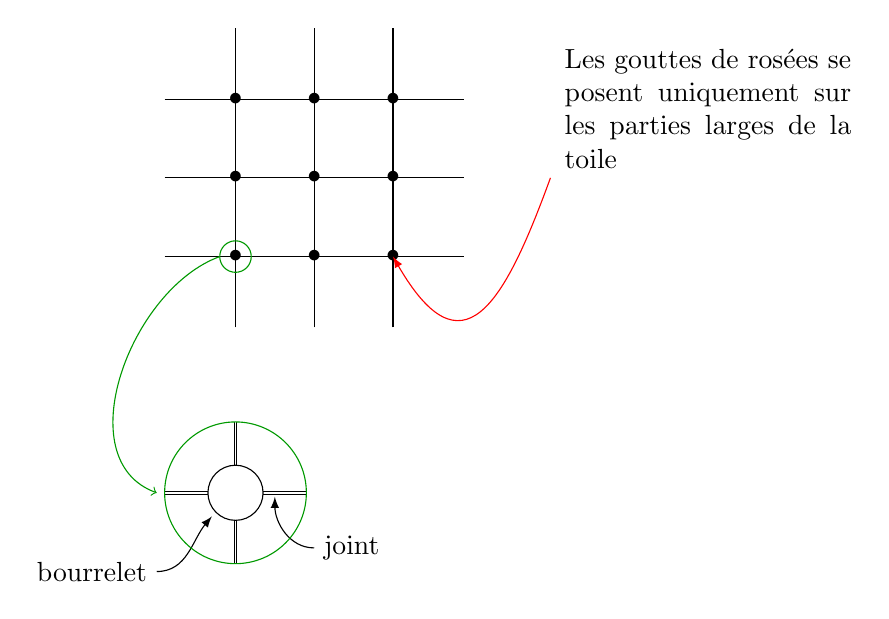
\begin{tikzpicture}
\draw (0.1,0.1) grid (3.9,3.9);
\foreach \j in {1,...,3}
    \foreach \i in {1,...,3}
    \draw (\i,\j) node{$\bullet$};
\draw[<-,>=latex, color=red] (3,1) to[out=-60, in=250, looseness=2] (5,2) node[above, xshift=2cm]{
\begin{minipage}{.3\linewidth}
\color{black} Les gouttes de rosées se posent uniquement sur les parties larges de la toile
\end{minipage}
};
\draw[->,color=green!60!black] (0.8,1) to[out=200,in=160,looseness=1] (0,-2);
\draw[color=green!60!black] (1,1)circle(0.2);

\begin{scope}[shift={(0,-3)}]
\draw[double] (0.1,0.1) grid (1.9,1.9);
\draw[fill=white](1,1) circle(0.35);
\draw[<-,>=latex](0.7,0.7) to[looseness=1, out=230, in=0] (0,0)node[left]{bourrelet};
\draw[<-,>=latex] (1.5,0.95) to[out=-90, in=180, looseness=1] (2,0.3) node[right]{joint};
\end{scope}
\draw[color=green!60!black] (1,-2) circle(0.9);
\end{tikzpicture}
$$


\underline{\textbf{Partie A :}} Etude des interactions intermoléculaires

\hspace{-1.5cm}\begin{minipage}{.6\linewidth}
\begin{tikzpicture}
  \begin{axis}[domain  = 0.5:2.3,
               samples = 100,
               xmin    = 0.3,
               xmax    = 2.3,
               ymin    = -1.4,
               ymax    = 1,
               xtick=\empty,
               ytick=\empty,
               xlabel  = {$r$},
               ylabel  = {$u$},
               extra y ticks = {0,-1},
               xlabel near ticks,
               ylabel near ticks,
               set layers,
              ] 
    \addplot[thick,
             samples=400
            ] {0.25/x^12-1/x^6};
    \draw[dashed,thin] (axis cs: 0.3, 0 )-- (axis cs: 2.3, 0);
    \draw[loosely dashed,very thin] (axis cs: 0.3, -1 )-- (axis cs: 2.3, -1);
\end{axis}
\end{tikzpicture}
\end{minipage}
\begin{minipage}{.5\linewidth}
\begin{enumerate}[label=\alph*)]
    \item Pourquoi $u\nearrow$ quand $r\to 0$ ?
    \item Quelle est la valeur de la distance de plus basse énergie ?
    \item Que se passe-t-il quand on éloigne deux atomes ?
\end{enumerate}
\end{minipage}

\bigskip

\begin{minipage}{0.3\linewidth}
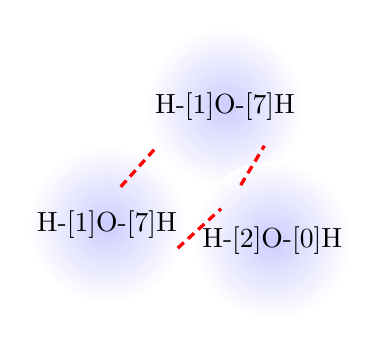
\begin{tikzpicture}
\shade[inner color=blue!20!white, outer color=white] (0,0) circle(1);
\draw(0,0) node{
\chemfig{H-[1]O-[7]H}
};
\shade[inner color=blue!20!white, outer color=white] (-1.5,-1.5) circle(1);
\draw(-1.5,-1.5) node{
\chemfig{H-[1]O-[7]H}
};
\shade[inner color=blue!20!white, outer color=white] (0.6,-1.7) circle(1);
\draw(0.6,-1.7) node[]{
\chemfig{H-[2]O-[0]H}
};

\draw[densely dashed, color=red, very thick] (-0.9,-.55)--(-1.35,-1.05);
\draw[densely dashed, color=red, very thick] (-0.6,-1.8)--(-.05,-1.3);
\draw[densely dashed, color=red, very thick] (.2,-1)--(0.5,-0.5);
\end{tikzpicture}
\end{minipage}
\begin{minipage}{.5\linewidth}
Interactions entre molécules d'eau (liaisons hydrogènes)
\end{minipage}

\hrulefill\\


\underline{\textbf{Partie B :}} On donne $W=\gamma S$ l'énergie de création d'une surface $S$ eau-air.

\begin{enumerate}[label=\alph*)]
    \item Justifier que créer une telle surface coûte de l'énergie
    \item On considère une goutte entre deux surfaces (bourrelet et joint). Montrer par un raisonnement énergétique sur un petit déplacement $dx$ qu'il existe une force sur la goutte d'eau.
\end{enumerate}

$$
\begin{tikzpicture}[scale=2]
    \draw(0,0)--++(0,2);
    \draw[pattern=north west lines] (0,1) circle(0.5);
    \draw[<->] (0,0.25)--++(.25,0) node[midway, below]{$dx$};
\end{tikzpicture}
$$

\hrulefill\\
\newpage

\underline{\textbf{Partie C :}} Pression de Laplace

$$
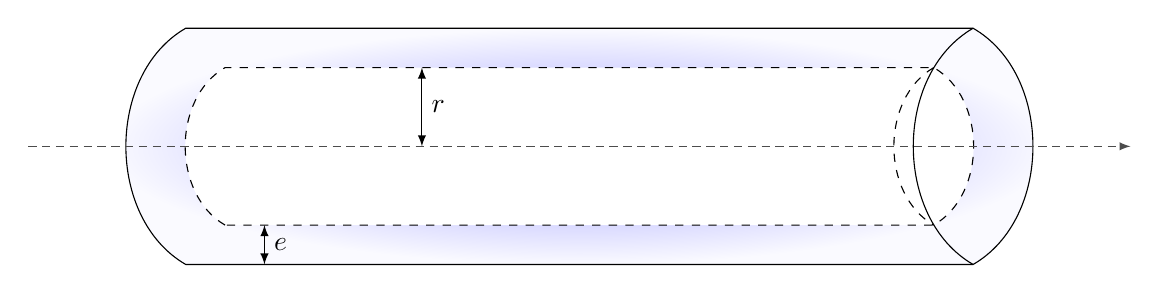
\begin{tikzpicture}
    \shade[inner color=blue!40!white, outer color=blue!2!white] (0,-1.5) to[out=150, in=-150, looseness=1] (0,1.5) --++(10,0) to[out=-30, in=30,looseness=1] (10,-1.5)--++(-10,0);
    
    \draw (0,-1.5) to[out=150, in=-150, looseness=1] (0,1.5) --++(10,0) to[out=-30, in=30,looseness=1] (10,-1.5)--++(-10,0);
    

    \draw[dashed, fill=white] (.5,-1) to[out=150, in=-150, looseness=1] (0.5,1) --++(9,0) to[out=-30, in=30,looseness=1] (9.5,-1)--++(-9,0);
    \draw[dashed] (9.5,1) to[out=-150, in=150, looseness=1](9.5,-1);

    \draw (10,1.5) to[out=-150, in=150, looseness=1](10,-1.5);
    
    \draw[<->,>=latex](1,-1.5)--++(0,.5) node[midway,right]{$e$};
    \draw[<->,>=latex] (3,0)--++(0,1) node[midway, right]{$r$};
    \draw[densely dashed, color=black!70!white,->, >=latex] (-2,0)--++(14,0);
    
\end{tikzpicture}
$$

On considère un cable tendu de rayon $r$, entouré d'une fine couche d'eau ($e$ très petit).\\
Montrer que la pression de la couche est telle que :

$$
\fbox{$P=\frac{\gamma_{a/r}}{r}$}
$$

\newpage